% Vector replica of Fig. 8 of the submitted manuscript (Fig8.jpeg, 1772 x 755 px); coordinates are the pixel
% positions of the original drawing (x right, y down), text and layout unchanged.
\documentclass[border=2pt]{standalone}
\usepackage[T1]{fontenc}\usepackage[scaled]{helvet}\renewcommand\familydefault{\sfdefault}
\usepackage{tikz}\usetikzlibrary{arrows.meta}
\definecolor{pr}{RGB}{252,0,0}\definecolor{gr}{RGB}{141,141,141}\definecolor{ge}{RGB}{90,90,90}
\definecolor{spyb}{RGB}{224,189,89}\definecolor{negb}{RGB}{28,91,124}
\begin{document}
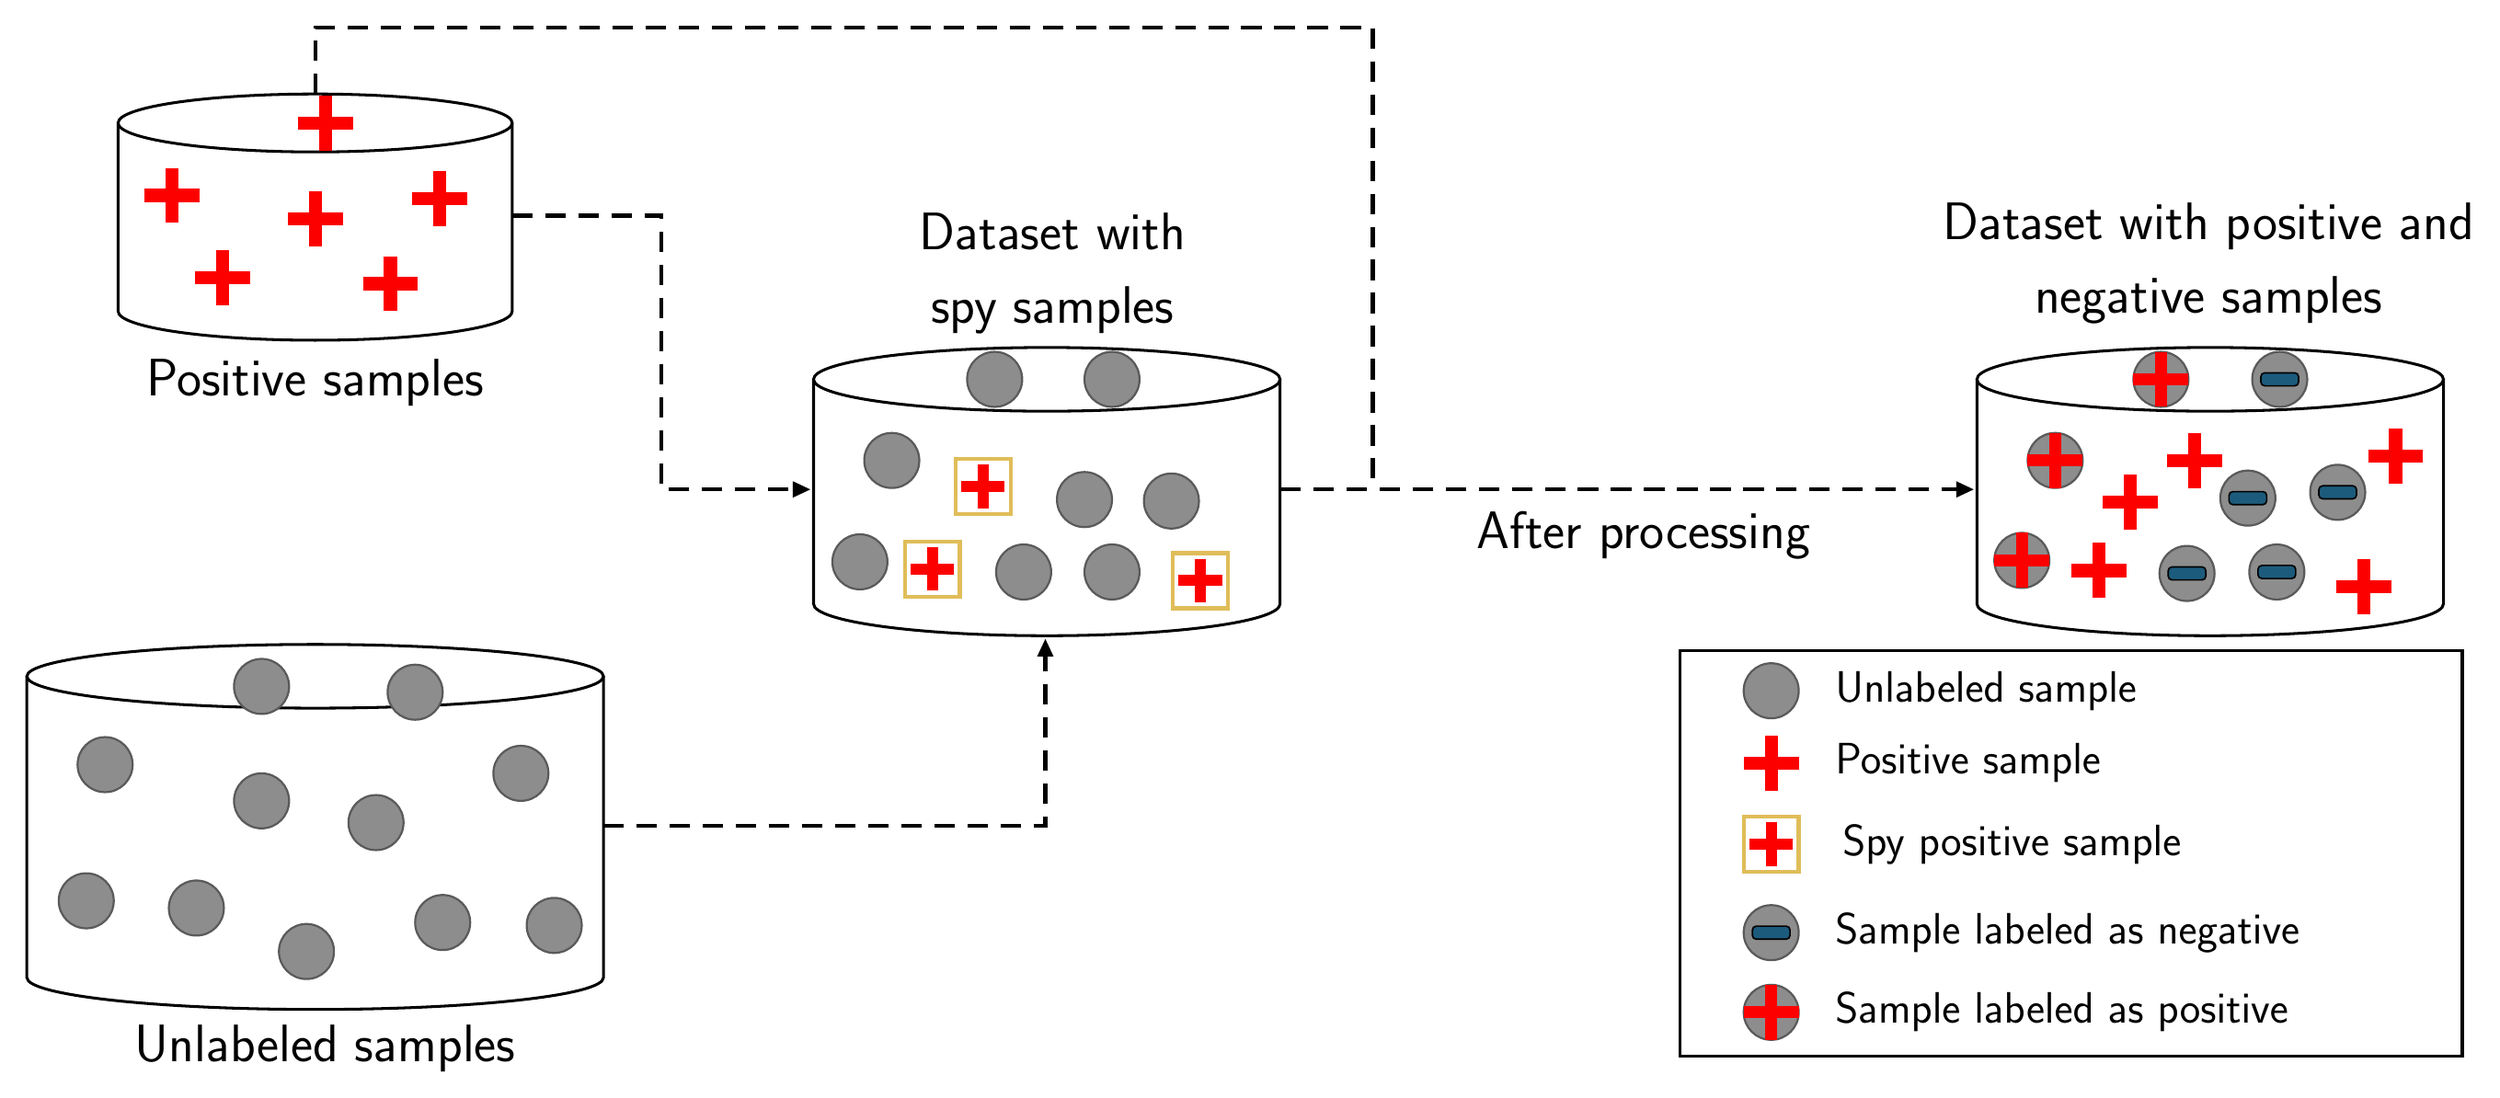
\begin{tikzpicture}[x=0.02cm, y=-0.02cm,
  tx/.style={align=center, font=\fontsize{21.5}{29}\selectfont, inner sep=0pt},
  lg/.style={anchor=west, font=\fontsize{18.5}{20}\selectfont, inner sep=0pt},
  dsh/.style={line width=1.5pt, dash pattern=on 8pt off 5pt},
  arr/.style={dsh, -{Triangle[length=7pt,width=6pt]}}]
% cylinder: x0, x1, top centre y, bottom centre y, ellipse half-height
\newcommand\cyl[5]{\fill[white] (#1,#3) -- (#1,#4) arc[start angle=180, end angle=0, x radius={(#2-#1)/2}, y radius=#5] -- (#2,#3) -- cycle;
  \draw[line width=1.1pt] (#1,#3) -- (#1,#4) arc[start angle=180, end angle=0, x radius={(#2-#1)/2}, y radius=#5] -- (#2,#3);
  \draw[line width=1.1pt, fill=white] ({(#1+#2)/2},#3) ellipse[x radius={(#2-#1)/2}, y radius=#5];}
\newcommand\plus[2]{\fill[pr] (#1-19,#2-4.5) rectangle (#1+19,#2+4.5); \fill[pr] (#1-4.5,#2-19) rectangle (#1+4.5,#2+19);}
\newcommand\unl[2]{\draw[ge, line width=0.8pt, fill=gr] (#1,#2) circle (19);}
\newcommand\spy[2]{\draw[spyb, line width=1.6pt, fill=white] (#1-19,#2-19) rectangle (#1+19,#2+19);
  \fill[pr] (#1-15,#2-3.8) rectangle (#1+15,#2+3.8); \fill[pr] (#1-3.8,#2-15) rectangle (#1+3.8,#2+15);}
\newcommand\negs[2]{\unl{#1}{#2}\draw[black, line width=0.6pt, fill=negb, rounded corners=1.5pt] (#1-13,#2-4.5) rectangle (#1+13,#2+4.5);}
\newcommand\pos[2]{\unl{#1}{#2}\fill[pr] (#1-19,#2-4.2) rectangle (#1+19,#2+4.2); \fill[pr] (#1-4.2,#2-19) rectangle (#1+4.2,#2+19);}
% arrows (drawn first, under the cylinders)
\draw[dsh] (236,68) -- (236,22) -- (966,22) -- (966,341);
\draw[arr] (372,152) -- (475,152) -- (475,341) -- (578,341);
\draw[arr] (435,573) -- (740,573) -- (740,444);
\draw[arr] (902,341) -- (1381,341);
% cylinders and contents
\cyl{100}{372}{88}{218}{20} \cyl{580}{902}{265}{420}{22} \cyl{1383}{1705}{265}{420}{22} \cyl{37}{435}{470}{678}{22}
\foreach \x/\y in {243/88,137/138,236/154,322/140,172/195,288/199} {\plus{\x}{\y}}
\foreach \x/\y in {705/265,786/265,634/321,767/348,827/349,612/391,725/398,786/398} {\unl{\x}{\y}}
\foreach \x/\y in {697/339,662/396,847/404} {\spy{\x}{\y}}
\foreach \x/\y in {1510/265,1437/321,1414/390} {\pos{\x}{\y}}
\foreach \x/\y in {1592/265,1570/347,1632/343,1528/399,1590/398} {\negs{\x}{\y}}
\foreach \x/\y in {1533/321,1489/350,1672/318,1467/397,1650/408} {\plus{\x}{\y}}
\foreach \x/\y in {199/477,305/481,91/531,199/556,278/571,378/537,78/625,154/630,230/660,324/640,401/642} {\unl{\x}{\y}}
% labels
\node[tx] at (236,267) {Positive samples};
\node[tx] at (745,192) {Dataset with\\spy samples};
\node[tx] at (1543,185) {Dataset with positive and\\negative samples};
\node[tx] at (243,727) {Unlabeled samples};
\node[tx] at (1153,373) {After processing};
% legend
\draw[line width=1.1pt] (1178,452) rectangle (1718,732);
\unl{1241}{480} \node[lg] at (1285,480) {Unlabeled sample};
\plus{1241}{530} \node[lg] at (1285,530) {Positive sample};
\spy{1241}{586} \node[lg] at (1290,586) {Spy positive sample};
\negs{1241}{647} \node[lg] at (1285,647) {Sample labeled as negative};
\pos{1241}{702} \node[lg] at (1285,702) {Sample labeled as positive};
\end{tikzpicture}
\end{document}
